%SourceDoc ../YourName-Dissertation.tex
%\vspace*{-80mm}
\chapter{Introduction} \label{chapter1:introduction}

\section{\sloppy Motivation}
Titanium (Ti) and its alloys have been used in biomedical applications for many years because of their biocompatibility and corrosion resistance properties \cite{Long1998a}. In recent years, there has been an increasing interest in developing better materials for load-bearing implants, due to the increase in total knee and hip replacements. Krutz et al. predicted that the total number of hip and knee replacements would increase by 174\% and 673\%, respectively, from 2005 to 2030, leading to 572,000 hip and 3.48 million knee procedures in the United States in 2030 \cite{Kurtz2007}. Two of the driving factors for this situation involve the increasing number of younger individuals requiring replacements and the fact that the average life of these implants is only about 7-12 years \cite{Krishna2007a}. These factors contribute significantly to the necessity for better implant materials. The primary considerations for biomedical implants, such as load-bearing knee and hip implants, are biocompatibility, corrosion resistance, fatigue strength, and Young's modulus ($E$) \cite{Long1998a}. In previous years, the most common implants for these applications have been Ti-6Al-4V, stainless steels, and MoCoCr alloys \cite{Niinomi2003,Niinomi2012}. However, there have been issues with these materials, such as cytotoxicity that has been observed with alloys containing aluminum and vanadium \cite{Ito1995a}. Another important impediment concerning the common implant materials is stress shielding, which can lead to implant failure. Stress shielding occurs when the $E$ of the implant is higher than that of bone. Due to the difference in $E$, load applications to the joint result in the implant material absorbing all of the stress and causing the bone surrounding the implant to atrophy, which leads to a loss in bone density, and can result in implant loosening and failure \cite{Long1998a}.  Table \ref{table:commonEM} summarizes the comparison of the $E$ of common implant materials (> 100 GPa) to bone (10-40 GPa) \cite{Long1998a} and shows the extreme elasticity mismatch between the various materials. Using computational thermodynamics to develop a knowledge base of Ti and its alloys is an extremely useful tool in overcoming these challenges.

This work focused on investigating the thermodynamic and elastic properties of the biocompatible Ti-Mo-Nb-Sn-Ta-Zr system. The thermodynamic and elastic properties were calculated using first-principles based on Density Functional Theory (DFT). The parametrization of the properties was completed using the CALPHAD modeling approach. The combination of these two methodologies has been shown to eliminate the need for trial-and-error metallurgy, thus saving time, money and resources. A new computational methodology to predict the metastable phase formation was presented and verified by neutron scattering experiments. The culmination of this work provides a fundamental understanding of the thermodynamics and elastic properties for the Ti-Mo-Nb-Sn-Ta-Zr system. 


\section{Overview}

The phase stability of Ti alloys has been shown to greatly affect the mechanical properties of these materials, so predicting and understanding this aspect of a Ti alloy will greatly impact its effectiveness as a biomedical implant.


\subsection{Equilibrium Phases}

Titanium is stable in the $\alpha$ (hexagonal close packed, hcp) phase (space group P$6_{3}/$mmc) under standard temperature and pressure. However, $\beta$ (body centered cubic, bcc) phase (space group Im$\overline{3}$m) Ti alloys have received a good deal of attention because of their low $E$ and high specific strength, so they have been targeted for biomedical applications \cite{Mei2011,Brailovski2011b}. Mo, Nb and Ta are biocompatible elements and strong $\beta$-stabilizers, while Zr is a bio-compatible weak $\beta$-stabilizer individually but strong stabilizer when in combination with other elements, such as Mo, Nb, and Ta \cite{Long1998a}. In conjunction with their biocompatiblity, studies have shown excellent Mo, Nb, Ta and Zr have excellent corrosion resistance and no allergy problems \cite{Tane2008a}. Recently, Sn has also been studied for use in Ti-alloys, due to its low cost \cite{Niinomi2012}. When alloyed in small concentrations, Sn does not effect the biocompability of the alloy. Therefore, the present study focused on determining the effects of alloying Ti with Mo, Nb, Sn, Ta and Zr on the thermodynamic properties. The combined DFT and CALPHAD approach was used to evaluate previous models and build new models for the binary and ternary alloys in the Ti-Mo-Nb-Sn-Ta-Zr system to build a completed database describing the thermodynamic properties of the system.

\subsection{Elastic Properties}

The mechanical properties, and phase stabilities have been experimentally determined for alloys such as Ti-13Nb-13Zr, Ti-35Nb-5Ta-7Zr-0.4O, Ti-29Nb-Ta-Zr and Ti-25Nb-Ta-Zr with Young's moduli between 71 and 57 GPa, approaching the $E$ of bone \cite{Long1998a,Tane2008a,Tane2010a}. While new metallic alloys are continually being designed, the ability to predict the elastic properties before attempting to develop alloys for biomedical implants will reduce the need for trial and error and narrow the sope of alloys being selected. In this dissertation, first-principles calculations were used to complete an extensive systematic study of the elastic properties of the pure elements, Ti-X systems and Ti-X-Y systems (X$\neq$Y=Mo,Nb,Sn,Ta,Zr) in the bcc phase. Multiple calculations were done across the entire composition range, using SQS to mimic the behavior of randomly substitued compositions. The first-principles results, were used to introduce interaction parameters that allow for the prediction of the elastic properties as a function of composition.

\subsection{Metastable Phases}

The completed thermodynamic database predicts the formation of the equilibrium phases, hcp and bcc. Based on the predictions, alloys that are in the bcc phase can be targeted and their elastic properties predicted. However, Ti and its alloys can form two metastable phases, $\alpha"$ and $\omega$. $\alpha"$ is an orthorhombic martensitic phase (space group Cmcm). The martensitic transformation is displacive \cite{Khachaturyan1985,Salje1990}. Thermodynamically the martensitic transformation is first-order and initiated by supercooling defined by $T_{0}-M_{S}$, where $T_{0}$ is the temperature where bcc transforms to hcp and $M_{S}$ is the temperature where the martensitic transformation begins. An applied stress can also contribute to the driving force for a martensitic transformation. Kinetically the martensitic transformation propagates in an athermal manner which suggests that the velocity of the interface and the force causing its movement contain an instability. The $\omega$ phase is a metastable hexagonal phase (space group P6/mmm) of Ti that has lattice parameters closely matching that of bcc Ti. The $\omega$ phase has been seen to form athermally when Ti is alloyed with $\beta$ stabilizing elements such as Mo, Nb and Ta. It has been shown that different cooling techniques of alloys at certain compositions in the Ti-Mo, Ti-Nb and Ti-Ta systems cause either the $\alpha"$ phase or the $\omega$ phase to form with a matrix of untransformed bcc phase. Quenching the samples leads to the formation of $\alpha"$, while slow cooling the samples leads to the formation of $\omega$ phase. The formation of theses phases causes variations to the predicted elastic properties as seen in Figure \ref{Ch1-figure:titaelastic} and \ref{Ch1-figure:tinbelasitc}, where the closed symbols represent the calculated $E$ and the open symbols represent the experimentally determined $E$ from the literature. The calculations and experiments agree well on the Ti-rich and Ta-rich sides but in the region marked by the purple box, the experiments show a higher $E$ than predicted by calculations. This is due to the formation of $\alpha"$ and $\omega$. While the formation of the metastable phases greatly effects the properties of the Ti-alloys, there is no current way to predict their formation. In this dissertation, a new theoretical framework was proposed to predict the formation. To introduce the theoretical framework and ensure the accuracy, the phase stability and effect on the elastic properties of the $\alpha"$ and $\omega$ phases were studied for the Ti-Nb and Ti-Ta systems. Initially, the ground state energy and elastic properties of multiple structures in the $\alpha"$, $\omega$, bcc and hcp were calculated, across all compositions, for the Ti-Ta and Ti-Nb systems. The new theoretic framework predicts the concentrations and phases fractions where the metastable phases form. The predicted phase fractions were then used to predict the $E$ using the rule of mixtures and mixed force constants are used to obtain the phonon density of states (DOS). The reults from inelastic neutron scattering were then used to determine diffraction patterns and phonon density of states. By looking at the diffraction patterns obtained at 300 $^\circ$K, the phase fractions were obtained and compared to the predicted phase fractions. The phonon DOS obtained from neutron scattering experiments at 300 $^\circ$K was compared with the mixed force constant first-principles phonon DOS. In order to study what type of transformation takes place for these metastable phases to form, the temperature dependence of the phonon DOS, obtained through neutron scattering, was analyzed. The predicted $E$ using the rule of mixtures was compared with experimental $E$ from literature.


\pagebreak
\section*{This completed thesis consists of the following main tasks:}

\begin{enumerate}
	\item The thermodynamics of the Ti-Mo-Nb-Sn-Ta-Zr system was investigated using first-principles calculations based on DFT and the CALPHAD method. 
	\begin{enumerate}
		\item Previous binary models were evaluated with the available experimental data as well as calculated enthalpy of formation of the bcc phase 
		\item The thermodynamic description of the Sn-Ta binary alloy was modeled
		\item The thermodynamic descriptions of the Ti-containing ternary alloys were modeled
	\end{enumerate}
	\item The elastic properties of the Ti-Mo-Nb-Sn-Ta-Zr system in the bcc phase were systematically calculated using first-principles based on DFT. The results were used to obtain interaction parameters, following the CALPHAD method, to predict the elastic properties as a function of composition. 
	\item The metastable phase formation in Ti alloys was investigated by first-principles calculations and experiments done on the Ti-Nb and Ti-Ta systems
	\begin{enumerate}
		\item The ground state energies and elastic properties of the Ti-Nb and Ti-Ta systems in the hcp, bcc, $\omega$ and $\alpha"$ were predicted using first-principles calculations
		\item From first-principles calculations:
			\begin{enumerate}
			\item The new theoretic framework was used to predict the phase fractions
			\item The phase fractions were used in a rule of mixtures to plot the phonon density of states and elastic properties
		\end{enumerate}
		\item From neutron scattering:
		\begin{enumerate}
			\item The phase fractions were determined and compared to the calculated predictions
			\item The phonon density of states, at 300 $^\circ$K, was compared to the mixed force constant predicted phonon density of states 
			\item The temperature dependent phonon density of states was used to study the transformation that occurs when these metastable phases form
		\end{enumerate}
	\end{enumerate} 
\end{enumerate}
				
\pagebreak
\begin{table}[H]
	\caption{Young's moduli of common implant materials compared with the Young's modulus of bone \cite{Long1998a}.}
	\centering
	\begin{tabular}{ c c }
		\hline
		Alloy & Young's Modulus (GPa) \\
		\hline
		Bone & 10-40\\
		cp-Ti* & 105\\
		Ti-6Al-4V & 110\\
		Stainless Steel & 200\\
		CoCrMo & 200-230\\
		\hline
		*cp-commercially pure titanium 
	\end{tabular}
\label{table:commonEM}
\end{table}
%%%
\clearpage

\newpage
%%%
\begin{figure}[H]
	\centering
	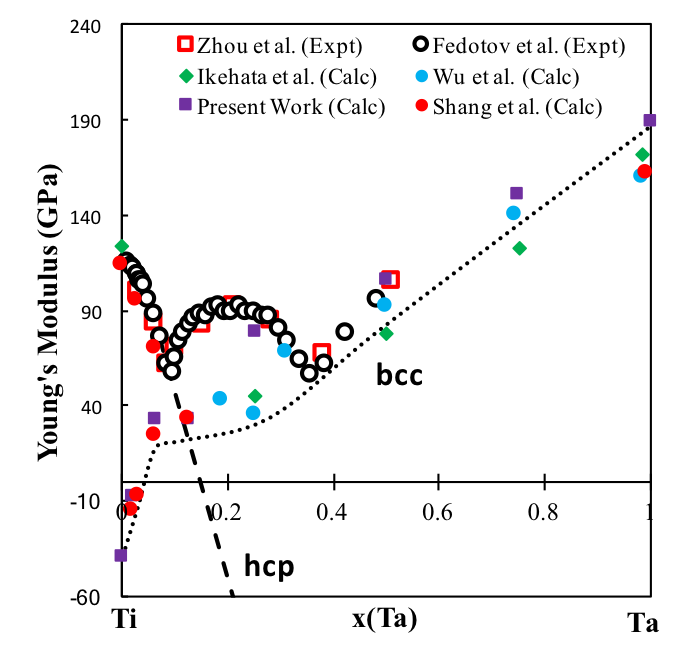
\includegraphics[width=\textwidth]{Chapter-1/Figures/TiTaElastic.png}
	\caption{Comparison of first-principles calculations \cite{Wu2010a,Ikehata2004} and experimental measurements of the Young's modulus of Ti-Ta alloys \cite{Zhou2004a,Zhou2009a,Fedotov1985}. The purple box refers to the composition range when the calculations and experimentally determined $E$ do not match up due to the formation of two metastale phases $\omega$ and $\alpha"$}
	\label{Ch1-figure:titaelastic}
\end{figure}
%%%

\newpage
%%%
\begin{figure}[H]
	\centering
	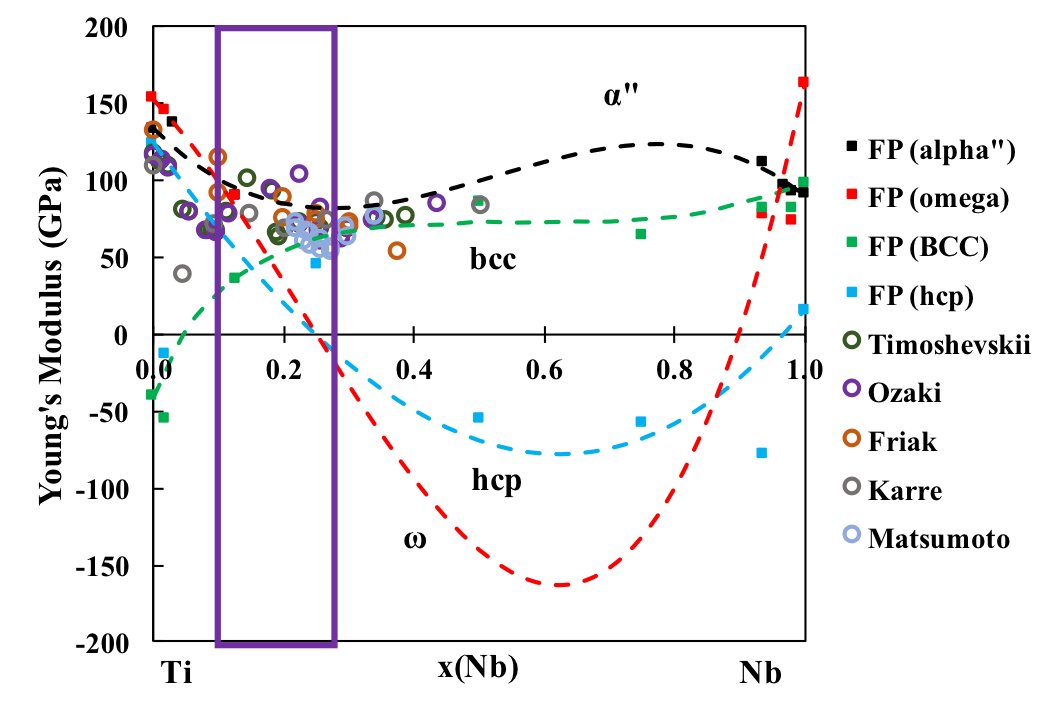
\includegraphics[width=\textwidth]{Chapter-1/Figures/TiNbElastic.png}
	\caption{Comparison of the present first-principles calculations and experimental measurements of the Young's modulus of Ti-Nb alloys \cite{Timoshevskii2011,Ozaki2004,Friak2012,Karre2015,Matsumoto2006}. The purple box refers to the composition range when the calculations and experimentally determined $E$ do not match up due to the formation of two metastale phases $\omega$ and $\alpha"$}
	\label{Ch1-figure:tinbelasitc}
\end{figure}
%%%
